
%\section{Multi-Agent Systems Review}
An essential concept which is repeatedly referred to in this thesis is that of an agent. The term "agent" is an abstract one with no single definition universally accepted in the literature. Most definitions agree reasonably closely with the one provided in AI: A Modern Approach by Russell and Norvig: an agent is "anything that can be viewed as perceiving its environment through sensors and acting upon that environment through actuators."\cite{AIAMA}.  Figure\ref{fig:agent_env_interaction} helps to illustrate this concept. \begin{figure}
    \centering
    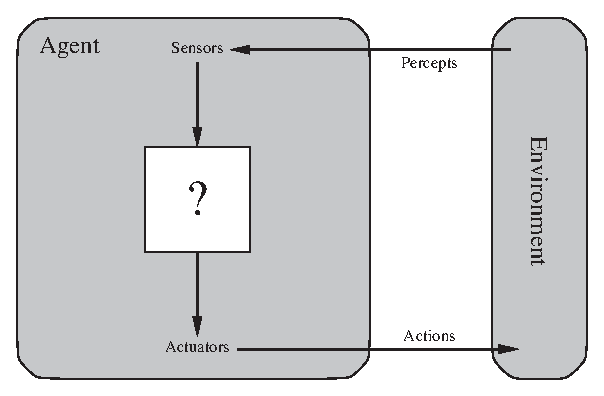
\includegraphics{Chapters/BackgroundKnowledgeAndRelatedWork/Figs/Vector/agent-environment.eps}
    \caption{Agent-Environment Interaction (Russell and Norvig)\cite{AIAMA}}
    \label{fig:agent_env_interaction}
\end{figure}
The box containing the question mark represents the agent's internal decision-making process, which generally speaking involves choosing an action, given the the complete history of everything that the agent has perceived. This action will be performed by the agent's actuators. The mapping from percept sequences to actions is described as the agent function. The agent function is an abstract notion; at a lower level an agent program implements the agent function, running on some physical system.\newline

When discussing agents, the following terms are commonly used to formally describe how the agent interacts with its environment: 
\begin{itemize}
    \item Environment States:
    \item Actions: The set of actions that the agent can choose to perform. 
    \item Percepts:
    \item Performance Measure:
    \item Goal
\end{itemize}



In order to design an agent function, certain desirable properties have been identified in the literature:
\begin{enumerate}
    \item Rationality: 
    \item Autonomy: 
    \item Reactivity: 
    \item Proactivity: 
\end{enumerate}


Agents are usually assumed to act in an environment, which comprises of everything external to the agent, which provides percepts and may change through actuation.

An agent is usually intuitively interpreted as an entity that acts on the behalf of a person on people in order to accomplish some high-level task.\par


To define a Multi-Agent System, it is instructive to first define the field from which it stems, Distributed Artificial Intelligence (DAI). A definition from Peter Stone states "DAI is concerned with systems that consist of multiple independent entities that interact in a domain."\cite{Stone2000MultiagentPerspective}
